\pdfminorversion=4
\documentclass[aspectratio=169]{beamer}

\mode<presentation>
{
  \usetheme{default}
  \usecolortheme{default}
  \usefonttheme{default}
  \setbeamertemplate{navigation symbols}{}
  \setbeamertemplate{caption}[numbered]
  \setbeamertemplate{footline}[frame number]  % or "page number"
  \setbeamercolor{frametitle}{fg=white}
  \setbeamercolor{footline}{fg=black}
} 

\usepackage[english]{babel}
\usepackage{inputenc}
\usepackage{tikz}
\usepackage{courier}
\usepackage{array}
\usepackage{bold-extra}
\usepackage{minted}
\usepackage[thicklines]{cancel}
\usepackage{fancyvrb}

\xdefinecolor{dianablue}{rgb}{0.18,0.24,0.31}
\xdefinecolor{darkblue}{rgb}{0.1,0.1,0.7}
\xdefinecolor{darkgreen}{rgb}{0,0.5,0}
\xdefinecolor{darkgrey}{rgb}{0.35,0.35,0.35}
\xdefinecolor{darkorange}{rgb}{0.8,0.5,0}
\xdefinecolor{darkred}{rgb}{0.7,0,0}
\definecolor{darkgreen}{rgb}{0,0.6,0}
\definecolor{mauve}{rgb}{0.58,0,0.82}

\title[2023-03-06-awkwardforth-for-atlas]{All about AwkwardForth}
\author{Jim Pivarski, Aryan Roy}
\institute{Princeton University, Manipal Institute of Technology}
\date{March 6, 2023}

\usetikzlibrary{shapes.callouts}

\begin{document}

\logo{\pgfputat{\pgfxy(0.11, 7.4)}{\pgfbox[right,base]{\tikz{\filldraw[fill=dianablue, draw=none] (0 cm, 0 cm) rectangle (50 cm, 1 cm);}\mbox{\hspace{-8 cm}
\includegraphics[height=1 cm]{princeton-logo-long.png}\hspace{0.1 cm}\raisebox{0.1 cm}{
\includegraphics[height=0.8 cm]{iris-hep-logo-long.png}}\hspace{0.1 cm}}}}}

\begin{frame}
  \titlepage
\end{frame}

\logo{\pgfputat{\pgfxy(0.11, 7.4)}{\pgfbox[right,base]{\tikz{\filldraw[fill=dianablue, draw=none] (0 cm, 0 cm) rectangle (50 cm, 1 cm);}\mbox{\hspace{-8 cm}
\includegraphics[height=1 cm]{princeton-logo.png}\hspace{0.1 cm}\raisebox{0.1 cm}{
\includegraphics[height=0.8 cm]{iris-hep-logo.png}}\hspace{0.1 cm}}}}}

% Uncomment these lines for an automatically generated outline.
%\begin{frame}{Outline}
%  \tableofcontents
%\end{frame}

% START START START START START START START START START START START START START

\begin{frame}{Introduction: what is AwkwardForth?}
\begin{center}
\begin{minipage}{0.89\linewidth}
\large\setlength{\baselineskip}{0.55 cm}

\vspace{0.5 cm}
AwkwardForth is an internal DSL within Awkward Array for accelerating sequential (non-columnar) data-ingest processes that must be discovered at runtime, avoiding a JIT-compilation toolchain as a dependency because Awkward Array is a foundational library.

\vspace{0.5 cm}
\uncover<2->{It has a stable API because an external package, Uproot, uses it heavily.}

\vspace{0.5 cm}
\uncover<3->{Because of all the qualifications in its justification, I doubt other projects would ever need it.}
\end{minipage}
\end{center}
\end{frame}

\begin{frame}{Conclusions}
\large
\begin{itemize}
\item You probably don't need it.
\end{itemize}
\end{frame}

\begin{frame}{\mbox{ }}
\Huge
\begin{center}
\textcolor{darkblue}{\bf BACKUP}
\end{center}
\end{frame}

\begin{frame}{Uproot-Awkward problem (for more-complex-than-jagged-arrays)}
\vspace{0.25 cm}
\only<1>{
\includegraphics[width=\linewidth]{PLOTS/awkward-uproot-interaction-1.pdf}}\only<2>{
\includegraphics[width=\linewidth]{PLOTS/awkward-uproot-interaction-2.pdf}}\only<3>{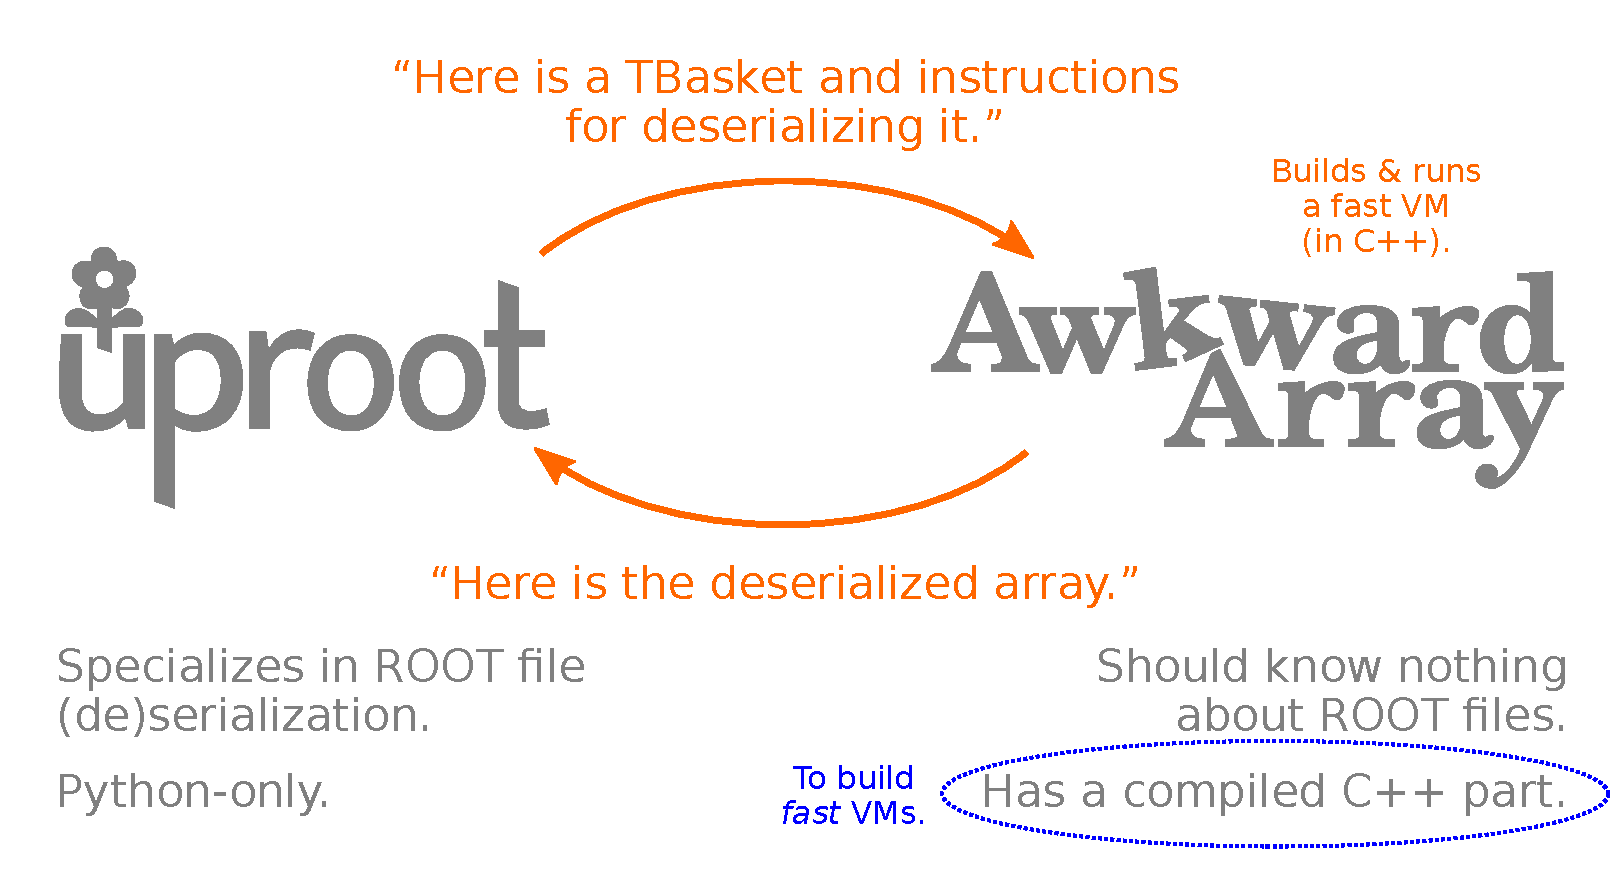
\includegraphics[width=\linewidth]{PLOTS/awkward-uproot-interaction-3.pdf}}
\end{frame}

\begin{frame}{We need a deserialization language; why Forth?}
\vspace{0.5 cm}
Forth was promoted in the early 1980's as an alternative to complex languages. It was the only language capable of running fast (compile-like speeds) within memory constraints of the first Macintosh.

\vspace{0.5 cm}
\begin{columns}
\column{0.5\linewidth}
\centering
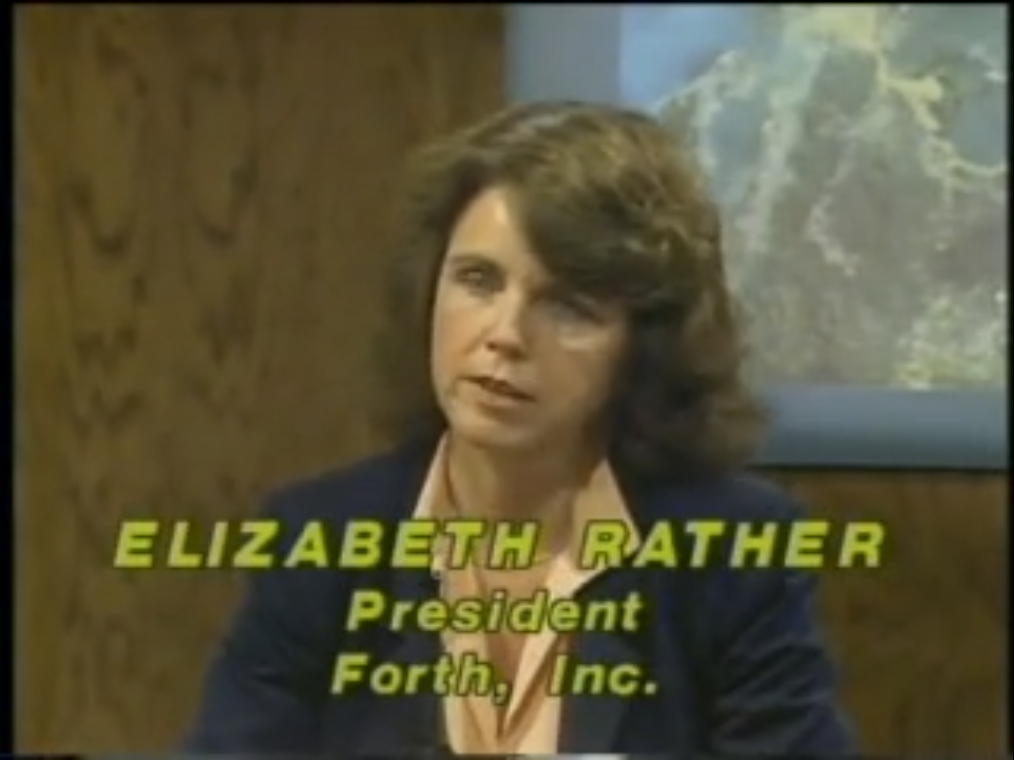
\includegraphics[height=5 cm]{PLOTS/elizabeth-rather-the-computer-chronicles.png}

\column{0.5\linewidth}
\centering
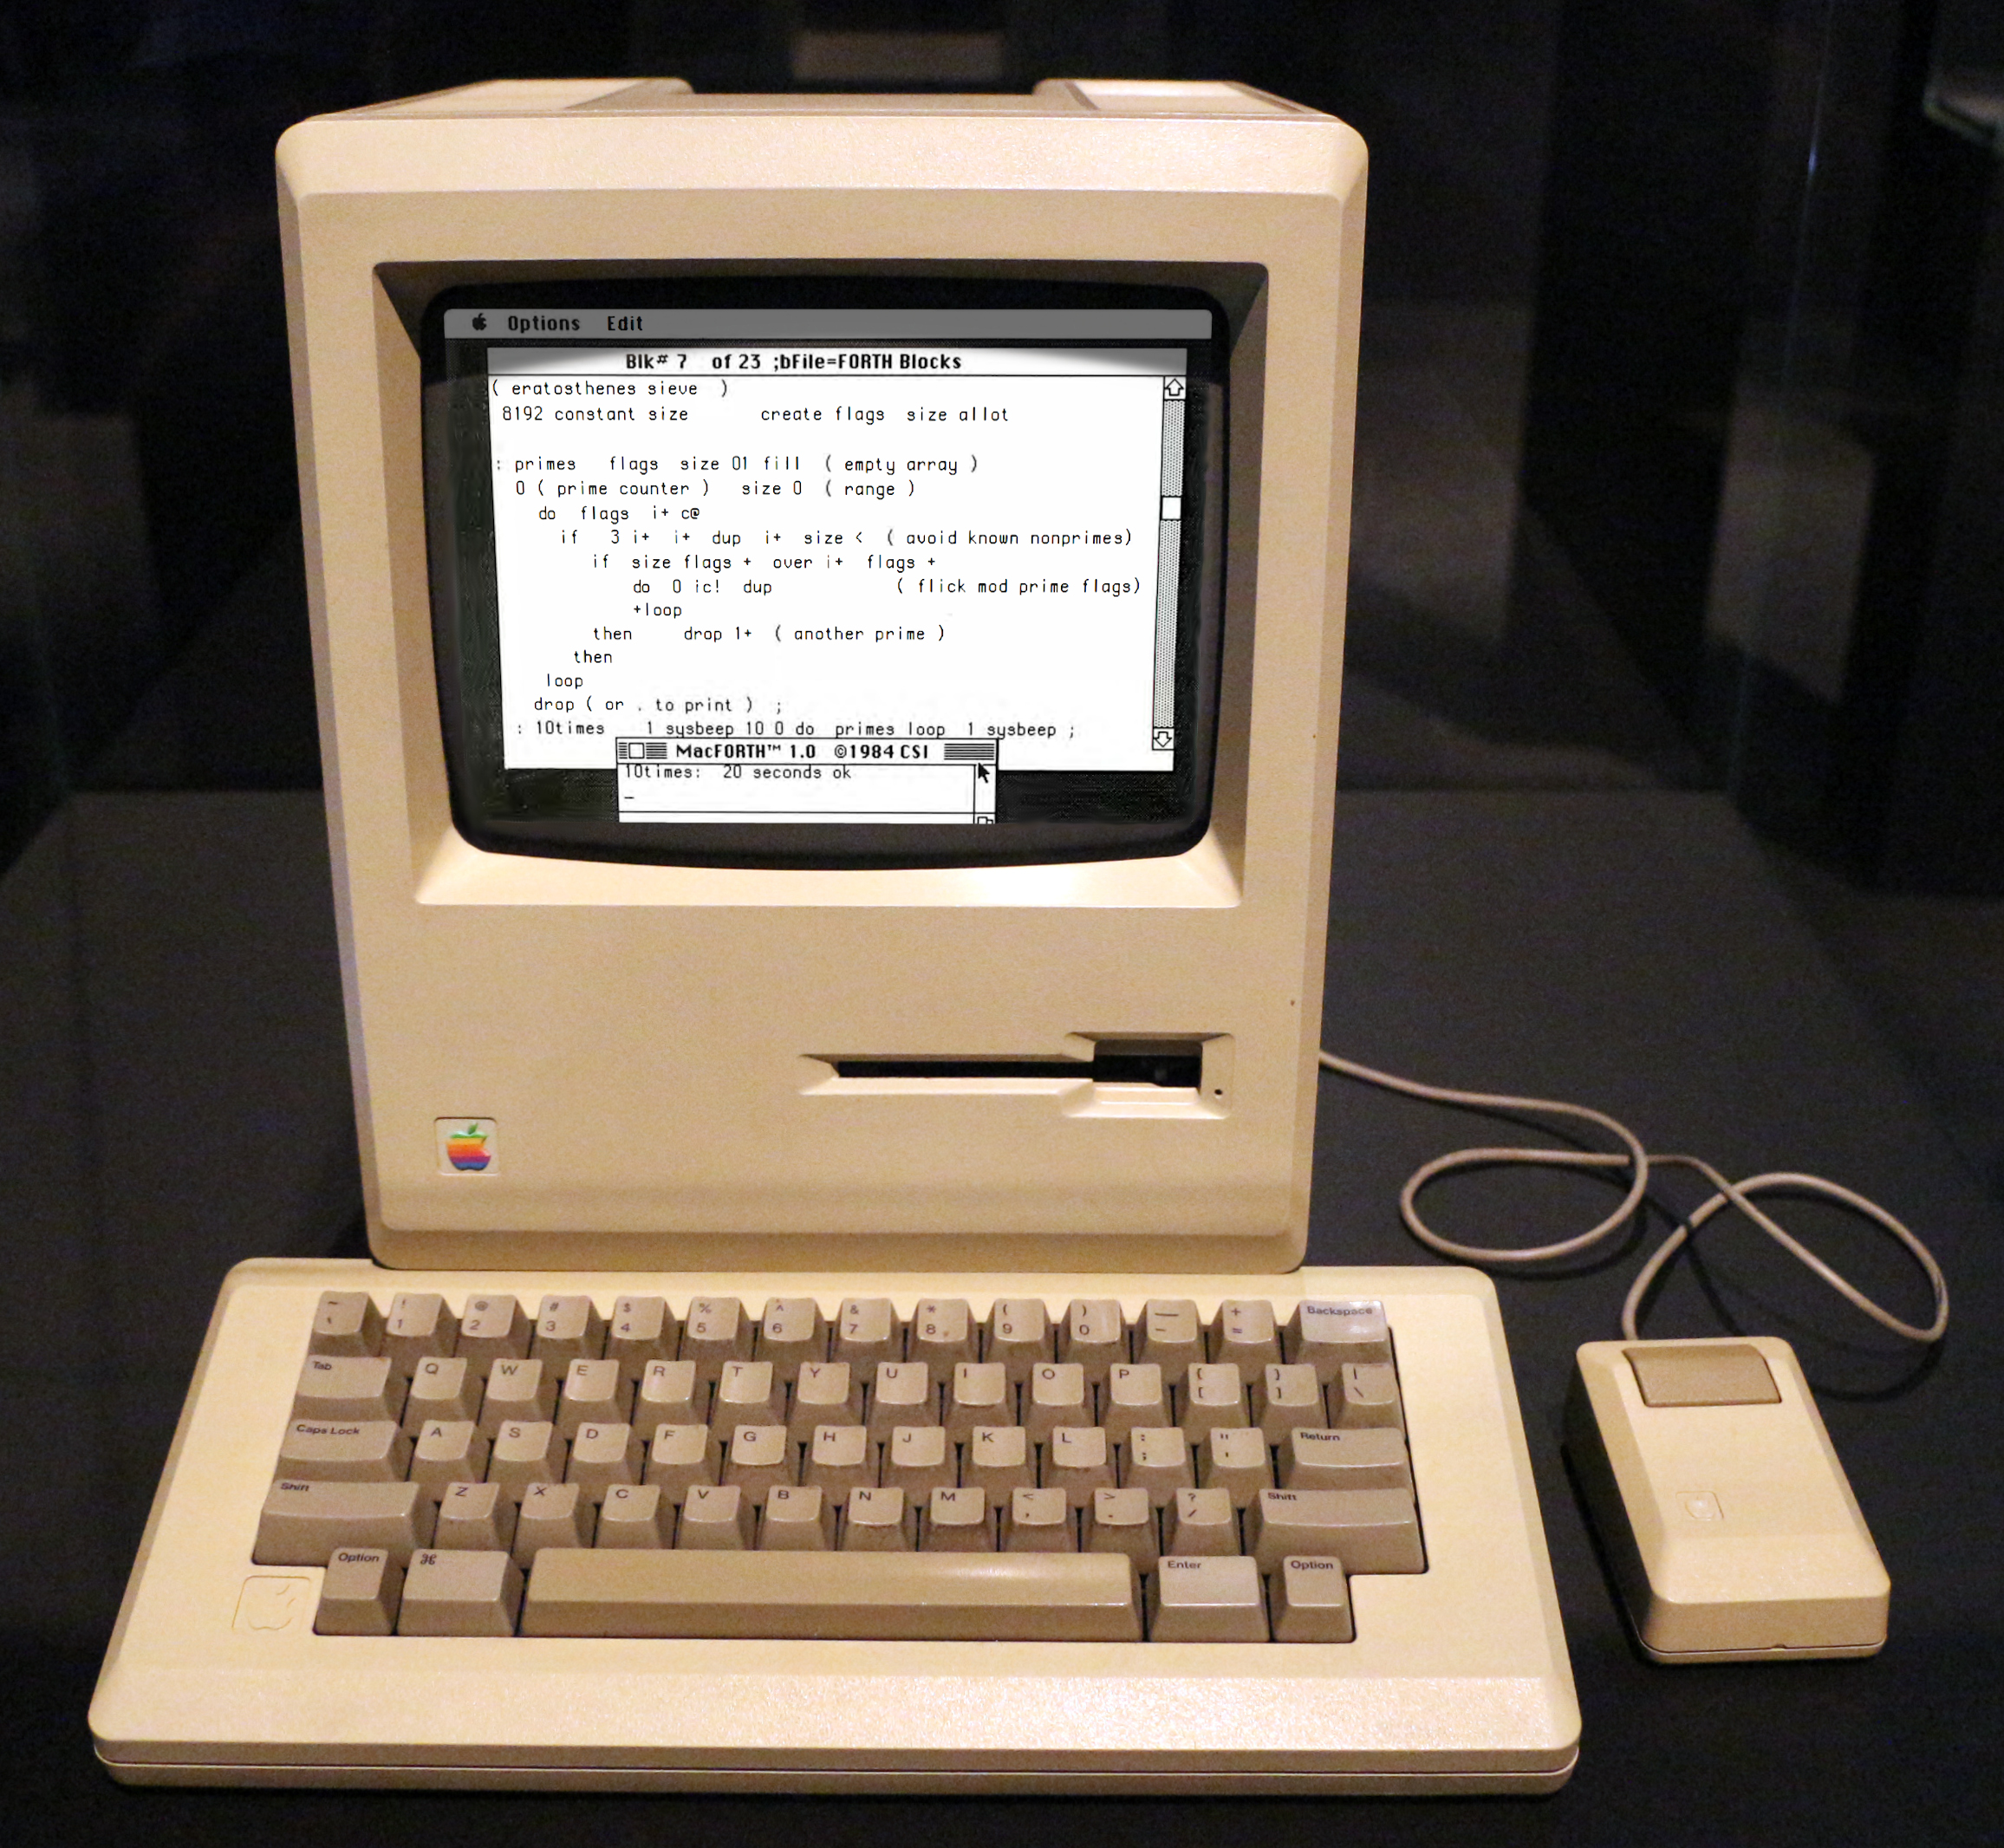
\includegraphics[height=5 cm]{PLOTS/macintosh-forth-code.jpg}
\end{columns}
\end{frame}

\begin{frame}{What Forth looks like (good for code generation!)}
\vspace{0.5 cm}
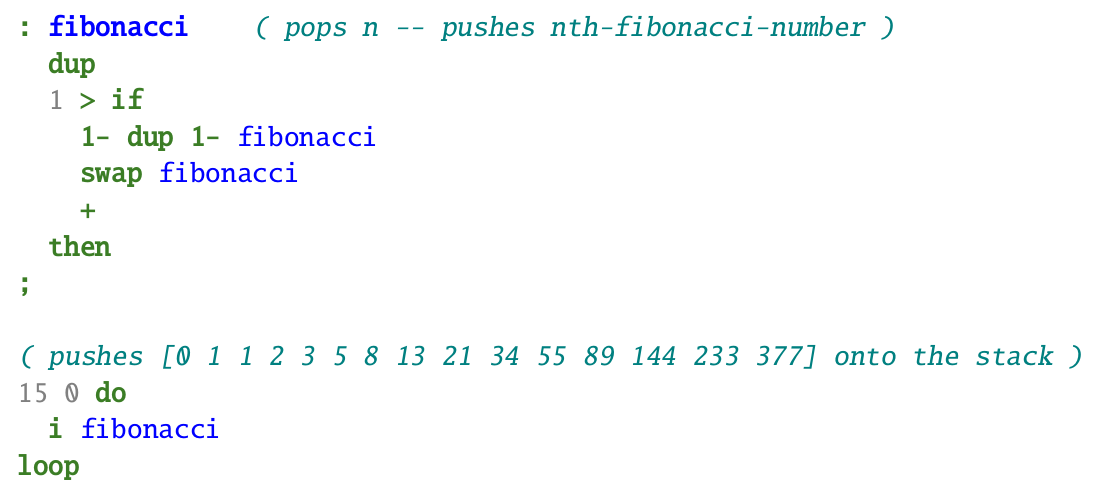
\includegraphics[width=0.9\linewidth]{PLOTS/forth-example.png}

\vspace{0.15 cm}
Almost no syntax; each whitespace-separated word performs an action on a stack of integers. This stack is the only data. Apart from the ability to define new words and the lack of jumps, it's essentially an assembler for a virtual stack-based machine.
\end{frame}

\begin{frame}{Adapted for data-ingest}
\vspace{0.25 cm}
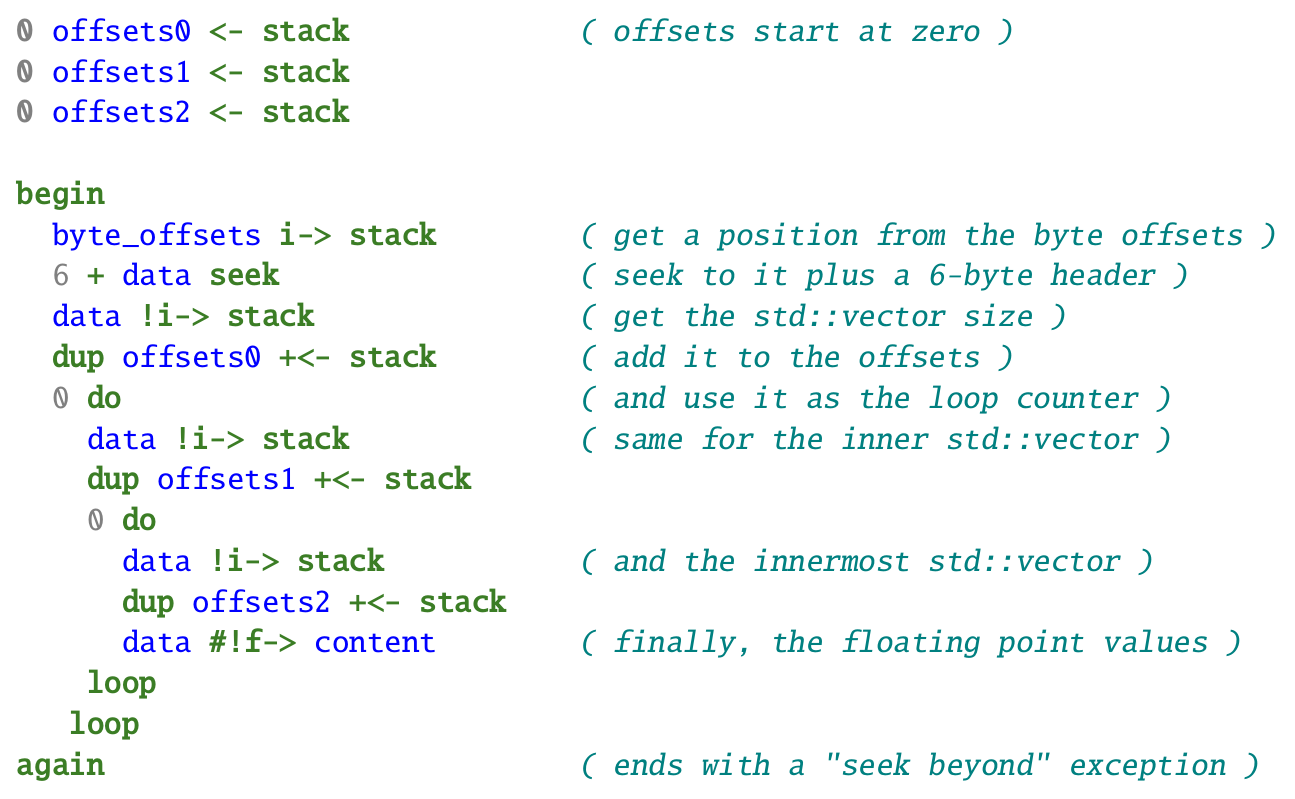
\includegraphics[width=0.9\linewidth]{PLOTS/forth-parsing-example.png}
\end{frame}

\begin{frame}{Summary of the argument}
\large
\vspace{0.25 cm}
\begin{enumerate}\setlength{\itemsep}{0.35 cm}
\item<1-> Uproot and Awkward need a way to talk to each other (neither are human).
\item<2-> Uproot expresses a procedure to turn bytes into Awkward Arrays.
\item<3-> Awkward needs to execute this procedure quickly.
\item<4-> We don't consider bundling a JIT-compiler into Awkward to be an option.
\item<5-> Forth is an {\it interpreted} language on a virtual machine, like Python, but it's so stripped down that it doesn't have most of the things that make Python slow. AwkwardForth instruction $\sim$5~ns, Python instruction $\sim$900~ns.
\item<6-> Bundling AwkwardForth in Awkward Array adds a few kilobytes without any dependencies. (Sssh! No one needs to know!)
\end{enumerate}
\end{frame}

\begin{frame}{The language was implemented 2 years ago}
\vspace{0.17 cm}
\begin{columns}
\column{1.15\linewidth}
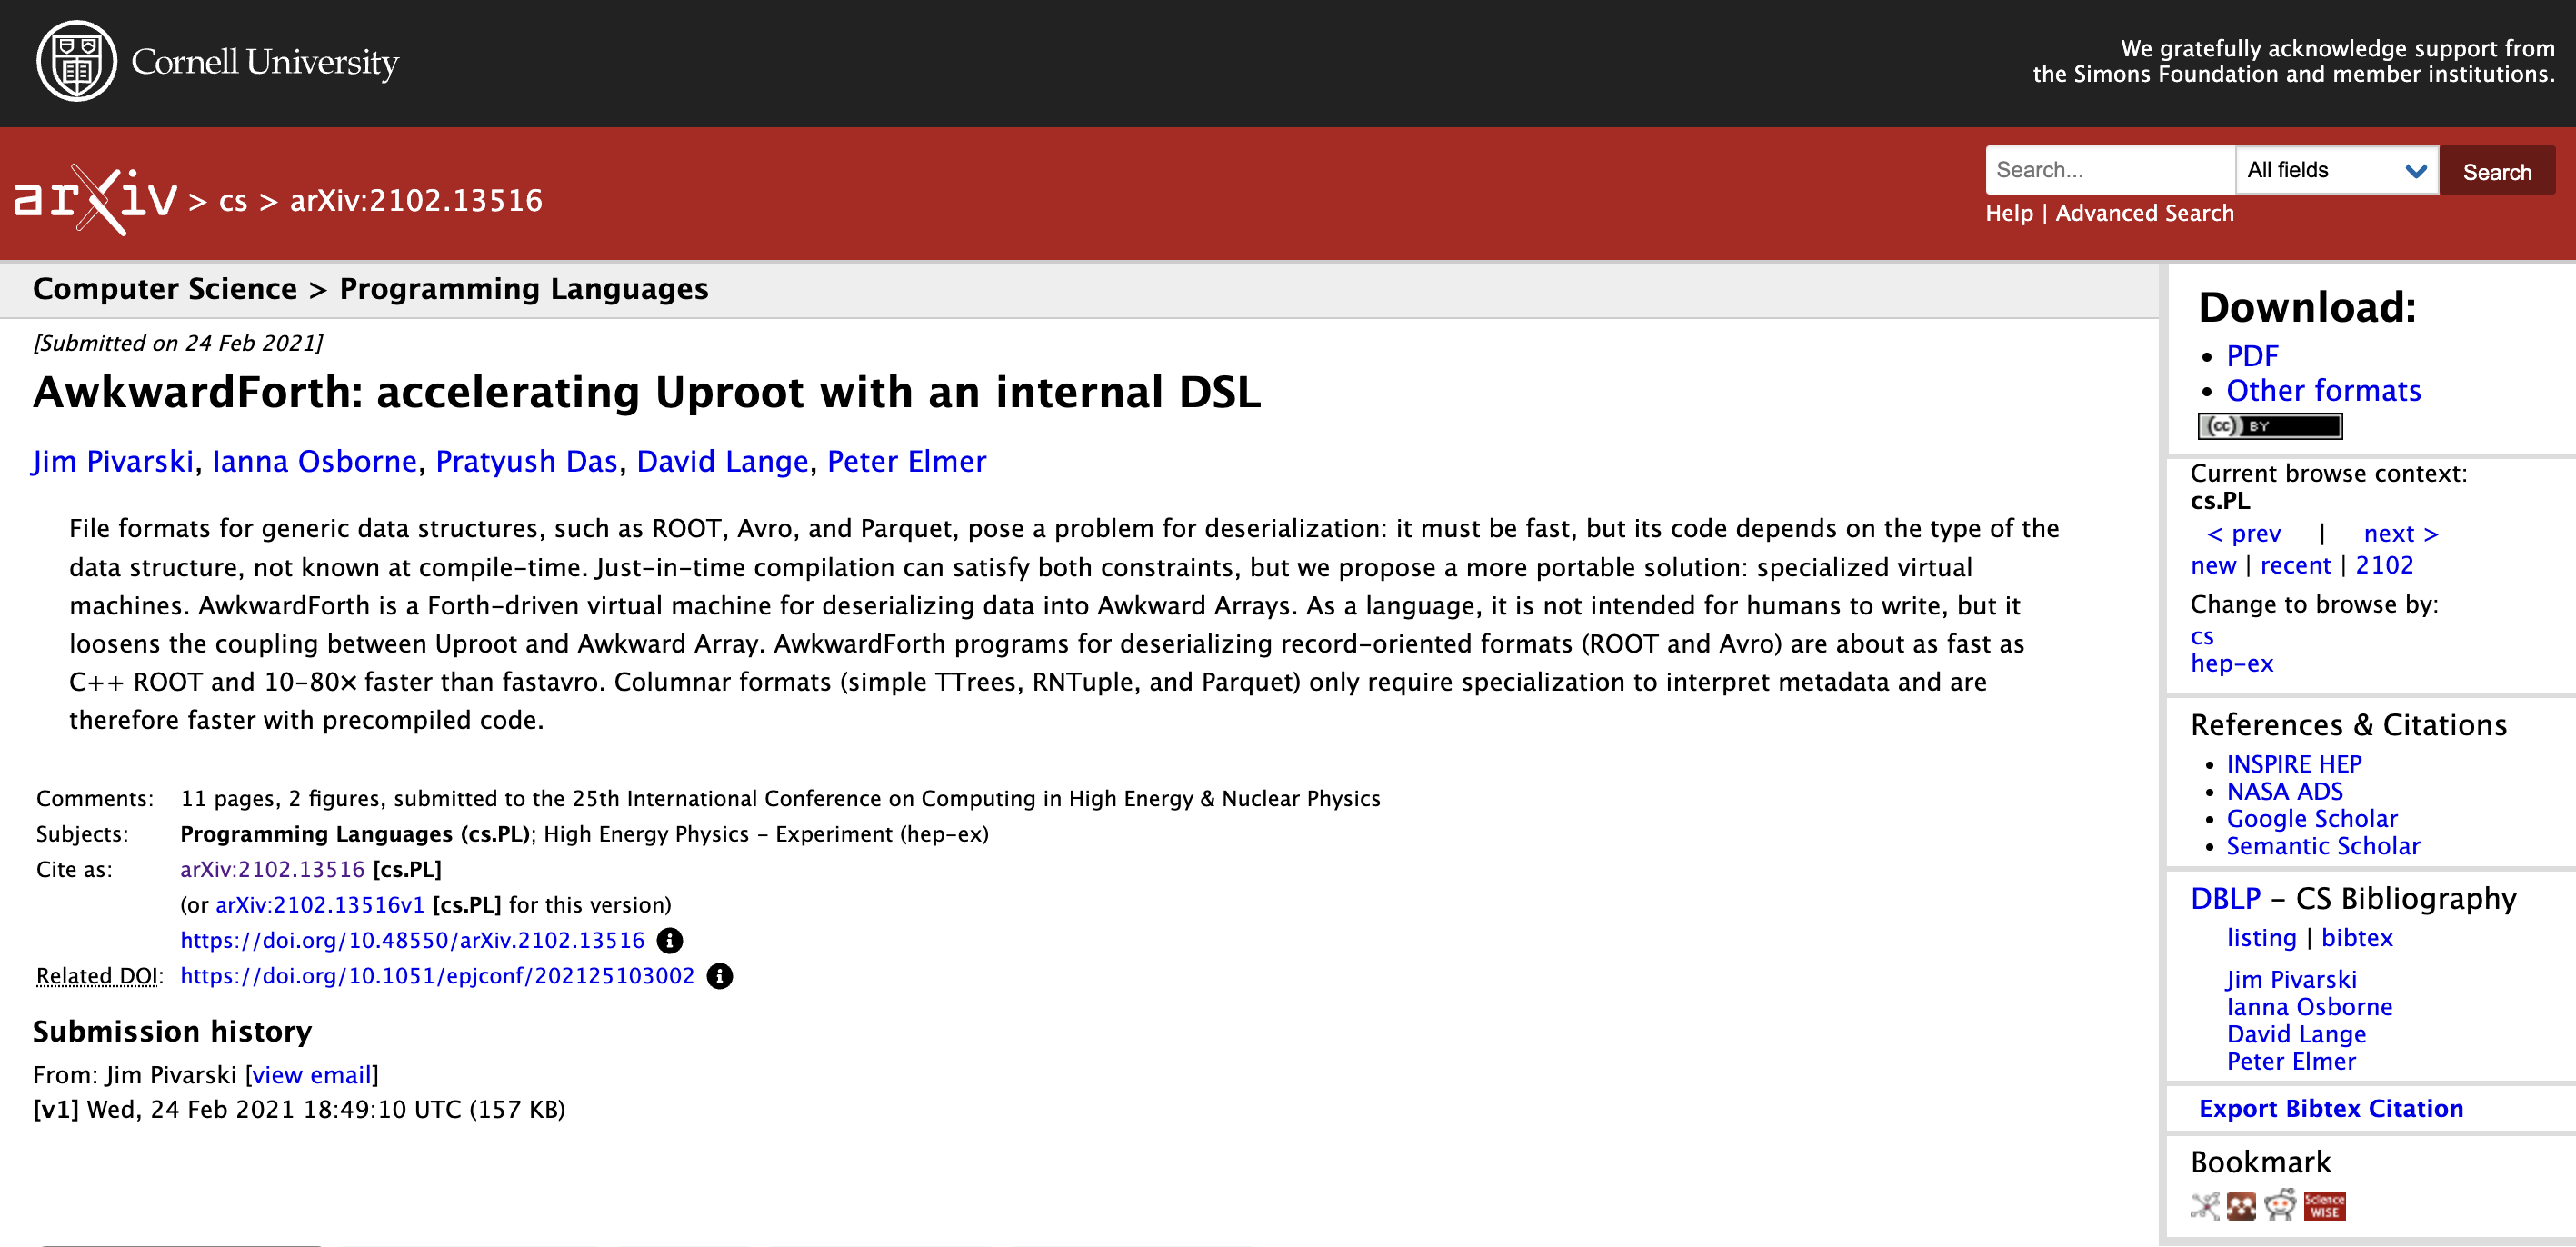
\includegraphics[width=\linewidth]{PLOTS/AwkwardForth-paper.png}
\end{columns}
\end{frame}

\begin{frame}{Uproot was updated to use it last summer (version 5.0)}
\vspace{0.17 cm}
\begin{columns}
\column{1.15\linewidth}
new paper here
\end{columns}
\end{frame}

\begin{frame}{The language is fully documented (so it's a stable API)}
\vspace{0.17 cm}
\begin{columns}
\column{1.15\linewidth}
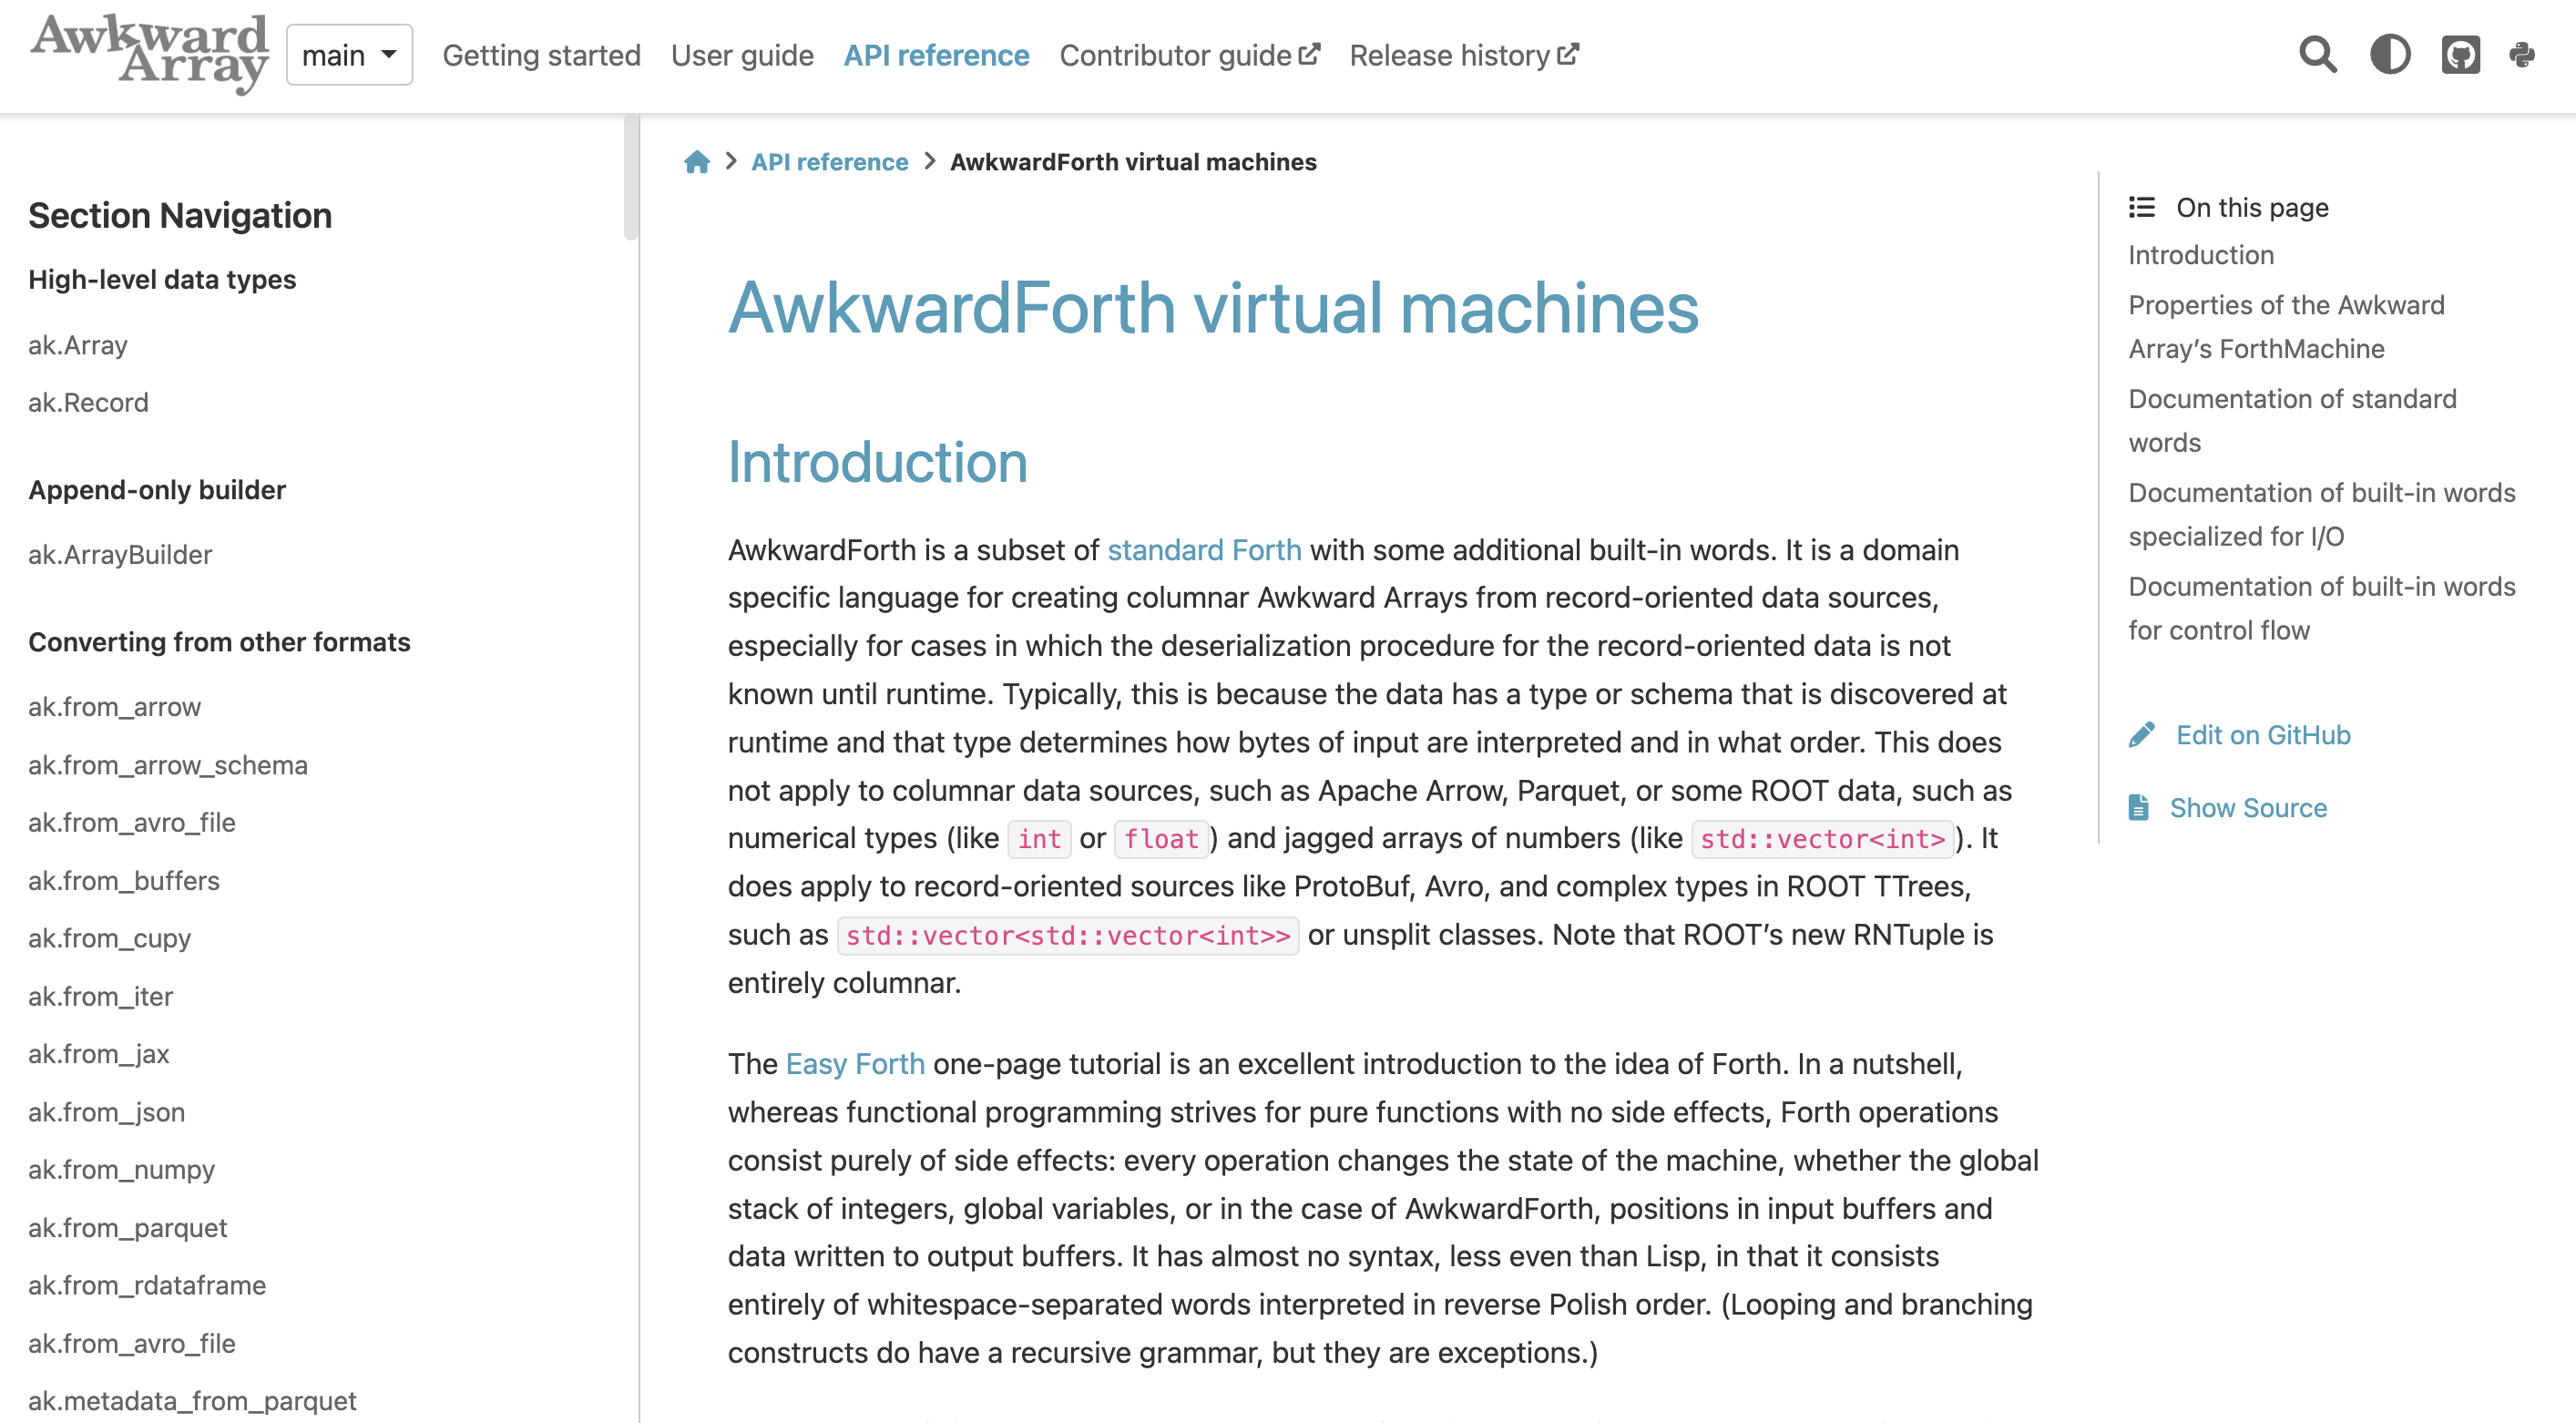
\includegraphics[width=\linewidth]{PLOTS/AwkwardForth-documentation.png}
\end{columns}
\end{frame}

\begin{frame}{Fixing Uproot's problem with non-columnar deserialization}
\vspace{0.25 cm}
\textcolor{darkorange}{\bf \centering This is the {\it predicted} performance (2 years ago, in proof-of-concept demo).}

\mbox{ } \hfill 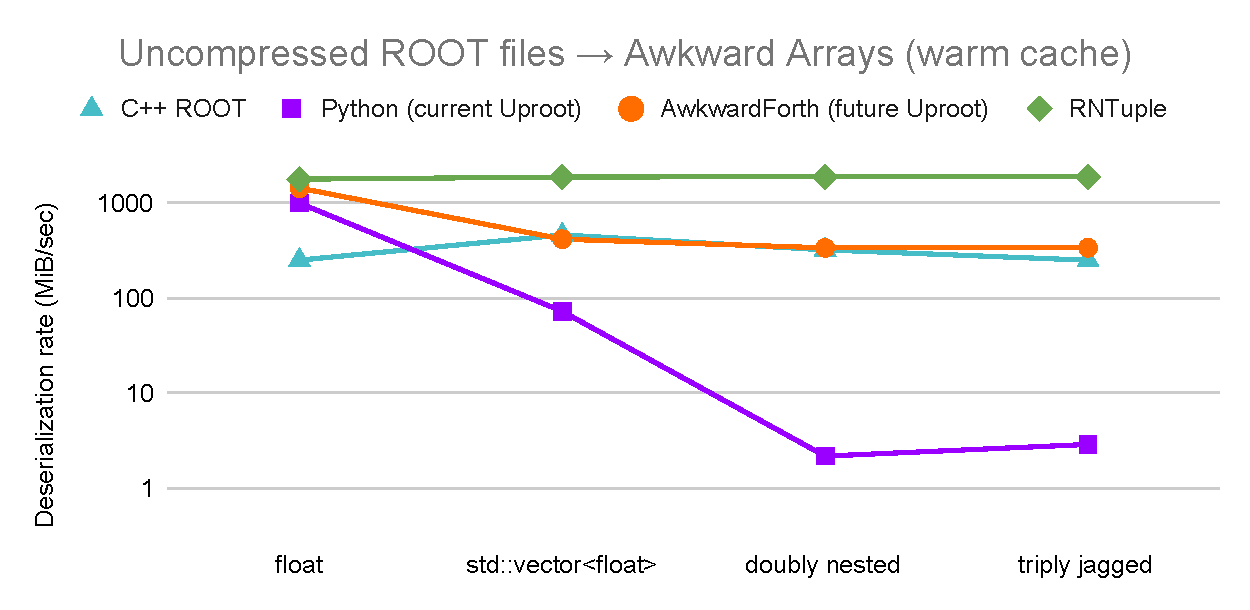
\includegraphics[width=0.9\linewidth]{PLOTS/AwkwardForth-performance-ROOT.pdf} \hfill \mbox{ }

Float and vector-of-float are columnar (and the purple point is 5$\times$ too low, a {\it mistake}).

Vector-of-vector-of-float and above are non-columnar.
\end{frame}

\begin{frame}{Fixing Uproot's problem with non-columnar deserialization}
\vspace{0.25 cm}
\textcolor{darkorange}{\bf \centering This is the {\it actual} performance (last summer, in Uproot itself).}

\mbox{ } \hfill 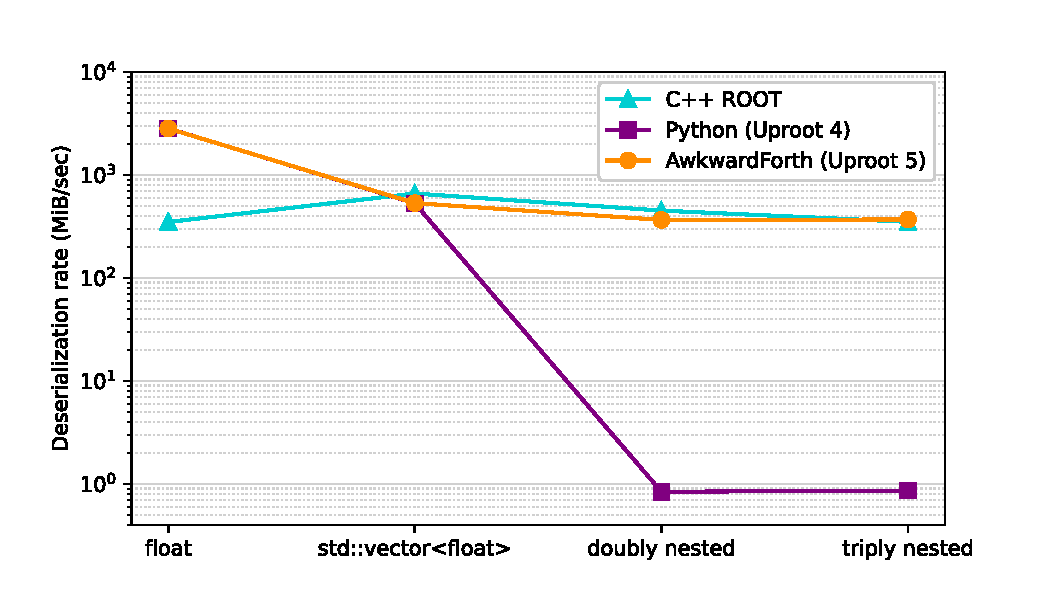
\includegraphics[width=0.9\linewidth]{PLOTS/awkwardforth-in-uproot-performance.pdf} \hfill \mbox{ }
\end{frame}

\begin{frame}{Scaling: AwkwardForth releases the Python GIL}
\vspace{0.25 cm}
\textcolor{darkorange}{\bf \centering This is the {\it predicted} performance (2 years ago, in proof-of-concept demo).}

\begin{columns}
\column{0.5\linewidth}
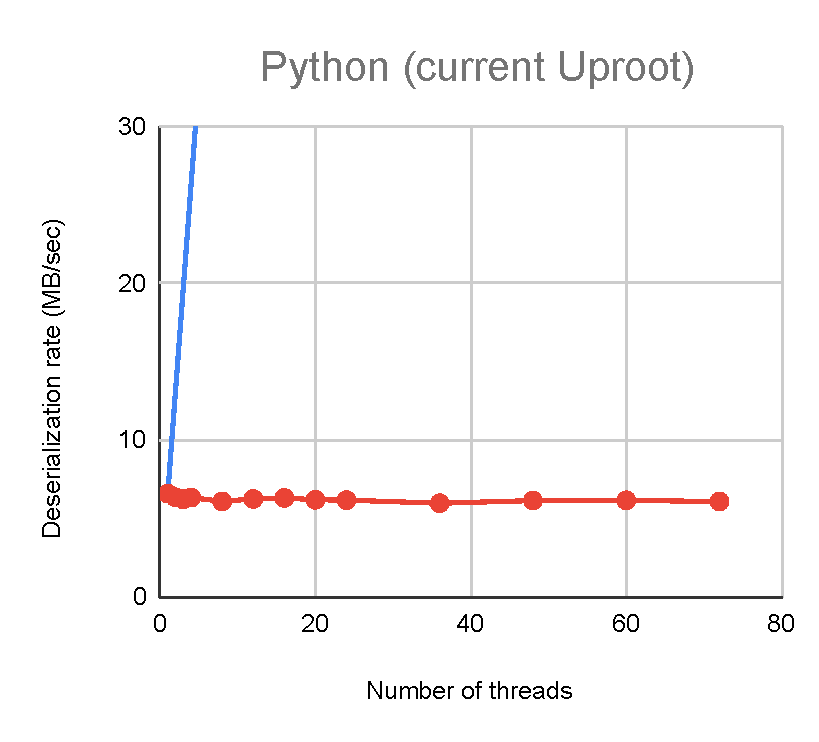
\includegraphics[width=\linewidth]{PLOTS/Python-scaling.pdf}

\column{0.5\linewidth}
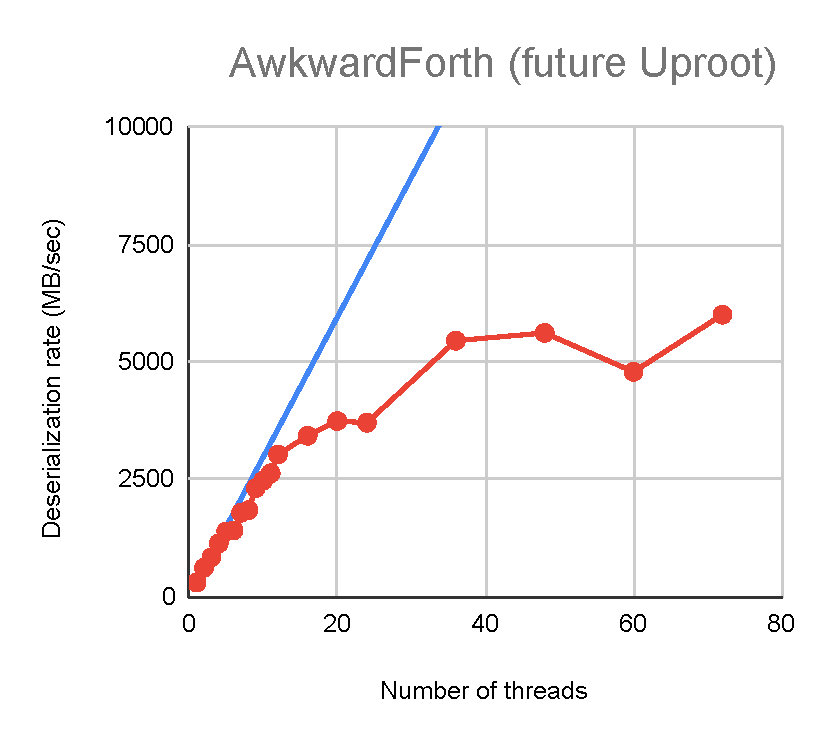
\includegraphics[width=\linewidth]{PLOTS/AwkwardForth-scaling.pdf}
\end{columns}
\end{frame}

\begin{frame}{Scaling: AwkwardForth releases the Python GIL}
\vspace{0.5 cm}
\textcolor{darkorange}{\bf \centering This is the {\it actual} performance (last summer, in Uproot itself).}

\vspace{-0.25 cm}
\mbox{\hspace{-1 cm}} 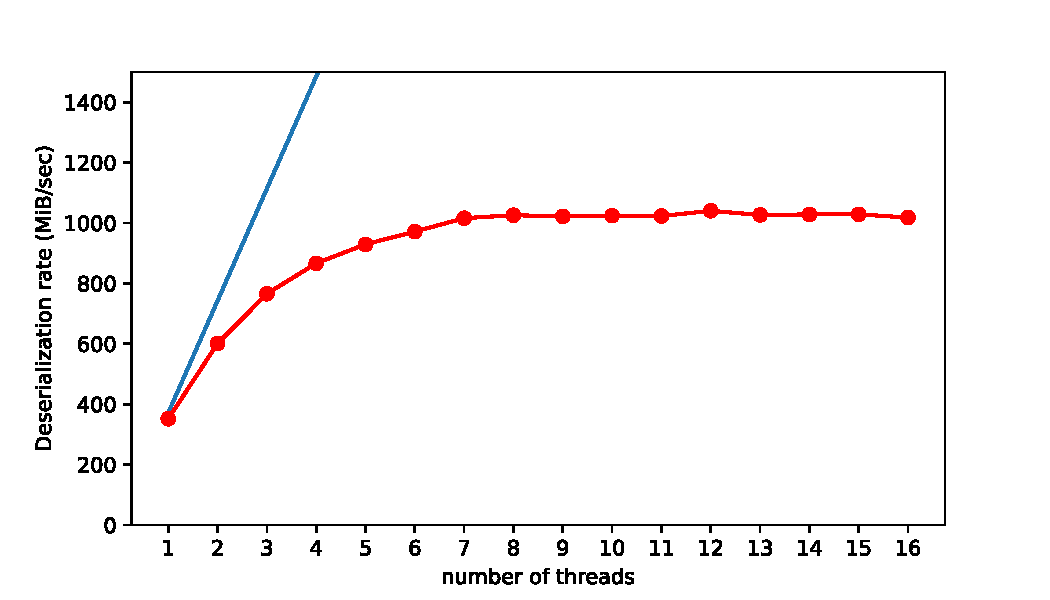
\includegraphics[width=0.7\linewidth]{PLOTS/awkwardforth-in-uproot-jagged3-scaling.pdf}

\vspace{-4 cm}
\hfill 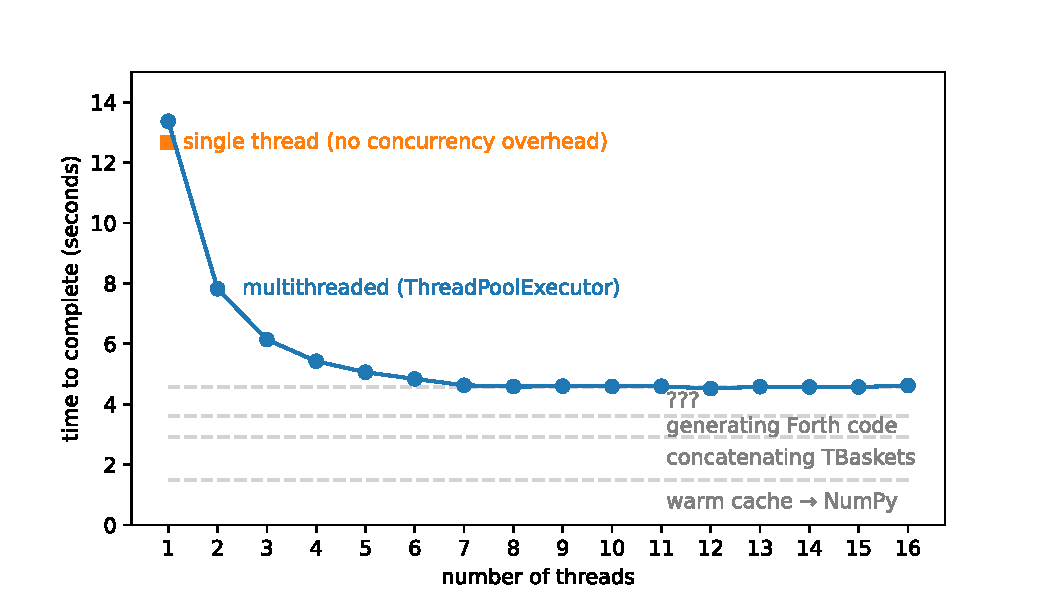
\includegraphics[width=0.7\linewidth]{PLOTS/awkwardforth-in-uproot-jagged3-scaling-reasons.pdf} \mbox{\hspace{-1.5 cm}}
\end{frame}

\begin{frame}[fragile]{What if we compile it anyway?}
\vspace{0.5 cm}
Some users have Numba (LLVM) installed.

\vspace{0.25 cm}
What if we convert AwkwardForth $\to$ Numba and let Numba compile it?

\vspace{0.5 cm}
Proof-of-concept implementation, given this test problem:

\vspace{0.25 cm}
Compute: $(x + 1) * (x - 2) + 3$

for $N$ iterations (i.e.\ no data flow).

\vspace{0.25 cm}
\fbox{\mintinline{forth}{dup 1 + swap 2 - * 3 +}}

\vspace{0.25 cm}
\scriptsize
\begin{minted}{ca65}
lea     eax, [rdi+1]
sub     edi, 2
imul    eax, edi
add     eax, 3
\end{minted}

\normalsize
\vspace{0.5 cm}
$\sim$1~second to compile, then 10$\times$ faster,

but only for arithmetically intensive code.

\vspace{-5.5 cm}
\hfill 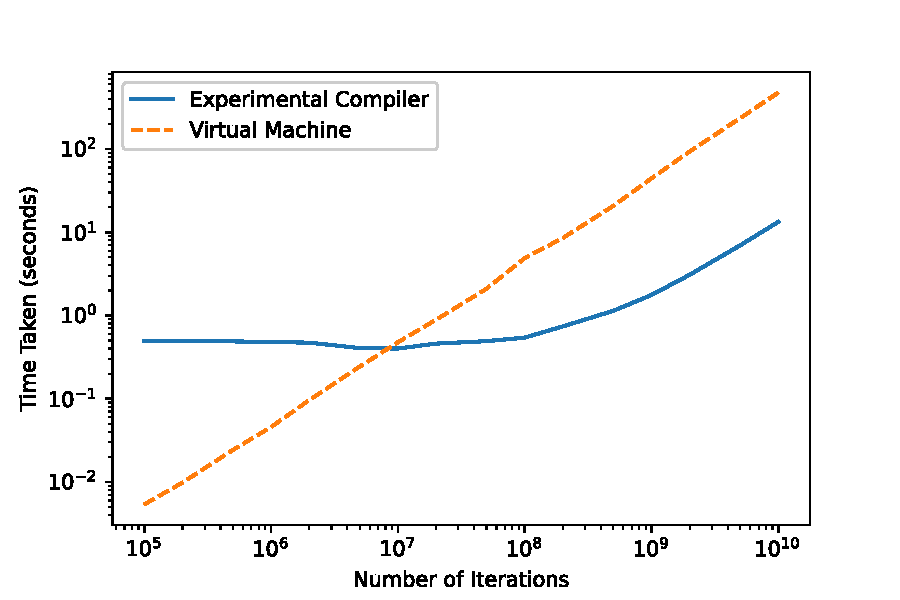
\includegraphics[width=0.6\linewidth]{PLOTS/new_compiler.pdf} \mbox{\hspace{-1 cm}}

\end{frame}


\end{document}
